\section{Overview}
In this work, we propose to steer the high-dimensional data exploration via local data analysis. It facilitates local data analysis in an efficient and distortion-free way.  In this section, we first illustrate the rationales for integrating local data analysis into interactive exploration. Then we

To be specific, the exploration contains four steps:
\begin{enumerate}[(1)]
 \item First, for any given projection, we help the user find a piece of interesting local data. Projection distortion and cluster suggestions are displayed to indicate potential outliers and clusters. The data chosen by user is called a 'focus', meaning that it's the current focus in local analysis.
 \item After some focus is chosen, we find its most featured projections for a targeted analysis. By 'features', we refer to three kinds of relationships we defined based on data distances. Projections are optimized to show these features with the least distortion.
 \item Since the focus is chosen in a projection, it could be a false cluster or missing some important pieces. We provide suggestions to help shape the focus into a more consistent and complete cluster. Whenever the focus is changed, the feature projections will also be updated.
 \item When some informative local data is found, the user can store it in a focus list. A 'projection map' is provided for all feature projections. It helps to compare different focuses, and navigate the high-dimensional exploration.
\end{enumerate}
 With our method, users are able to explore the data space efficiently, by analyzing different parts of local data in a distortion-free way.

\ifx
\begin{figure*}[htb]
\centering
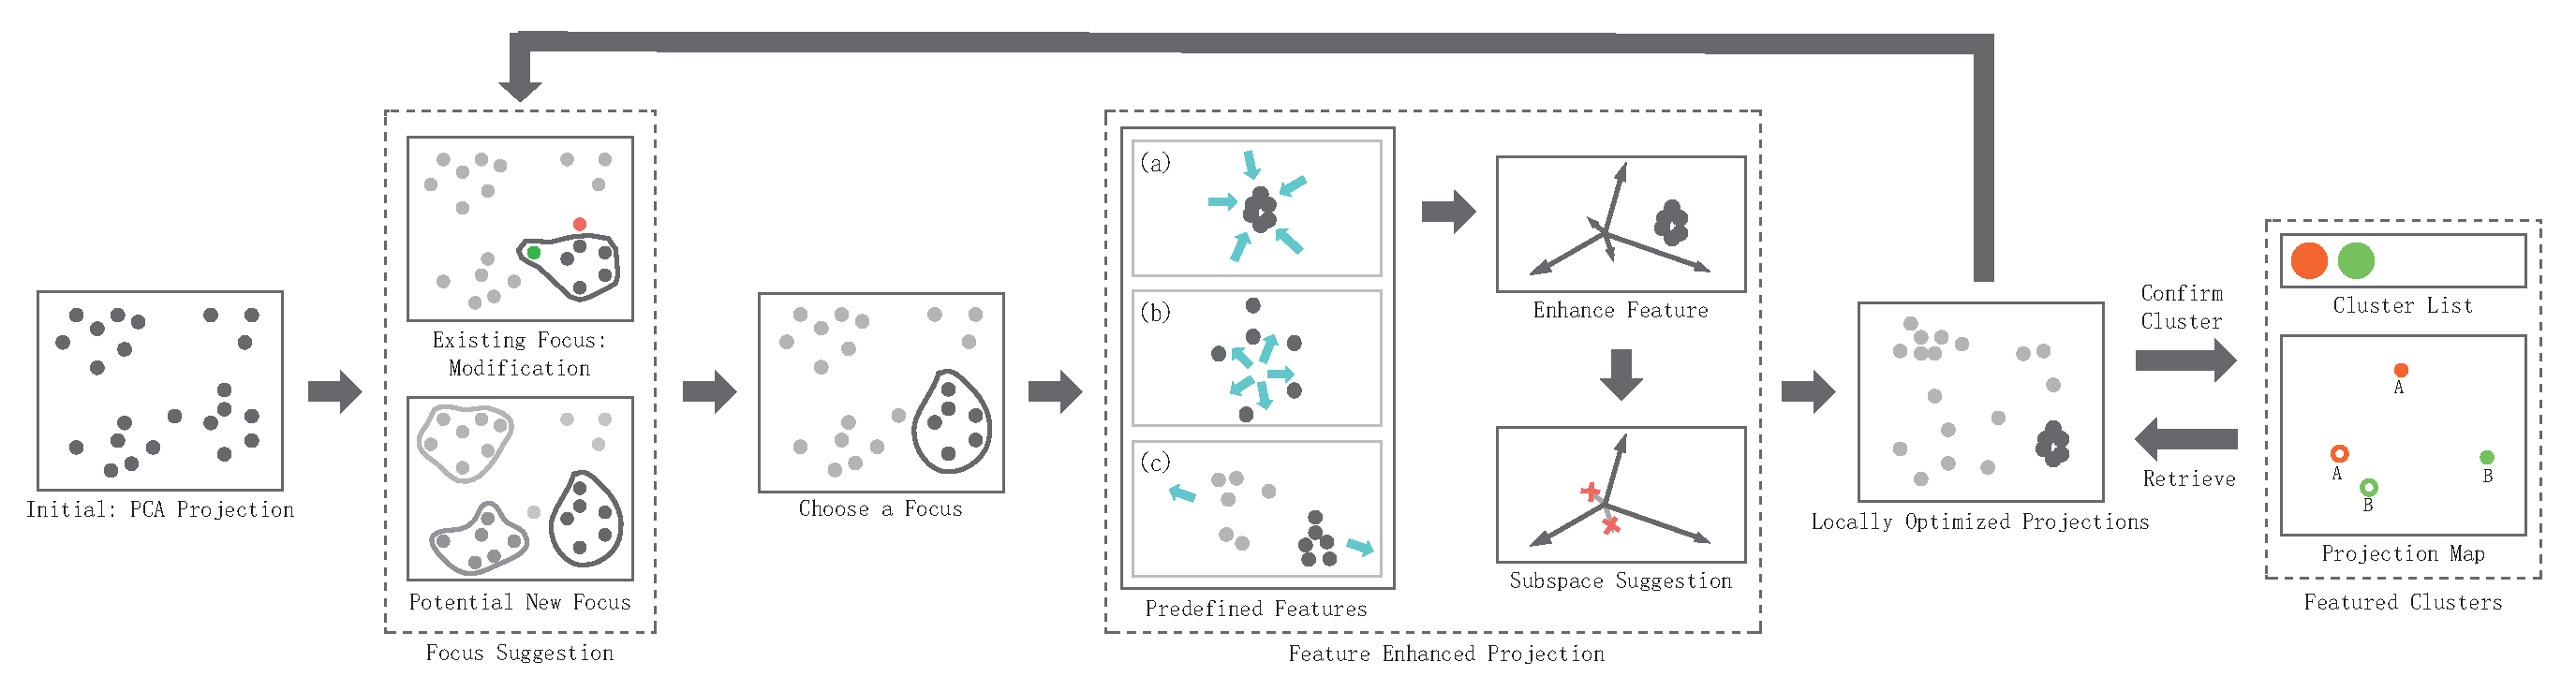
\includegraphics{images/Pipeline.eps}
\caption{Sample illustration.}
\end{figure*}
\else
\begin{figure*}[htbp]
\centering
  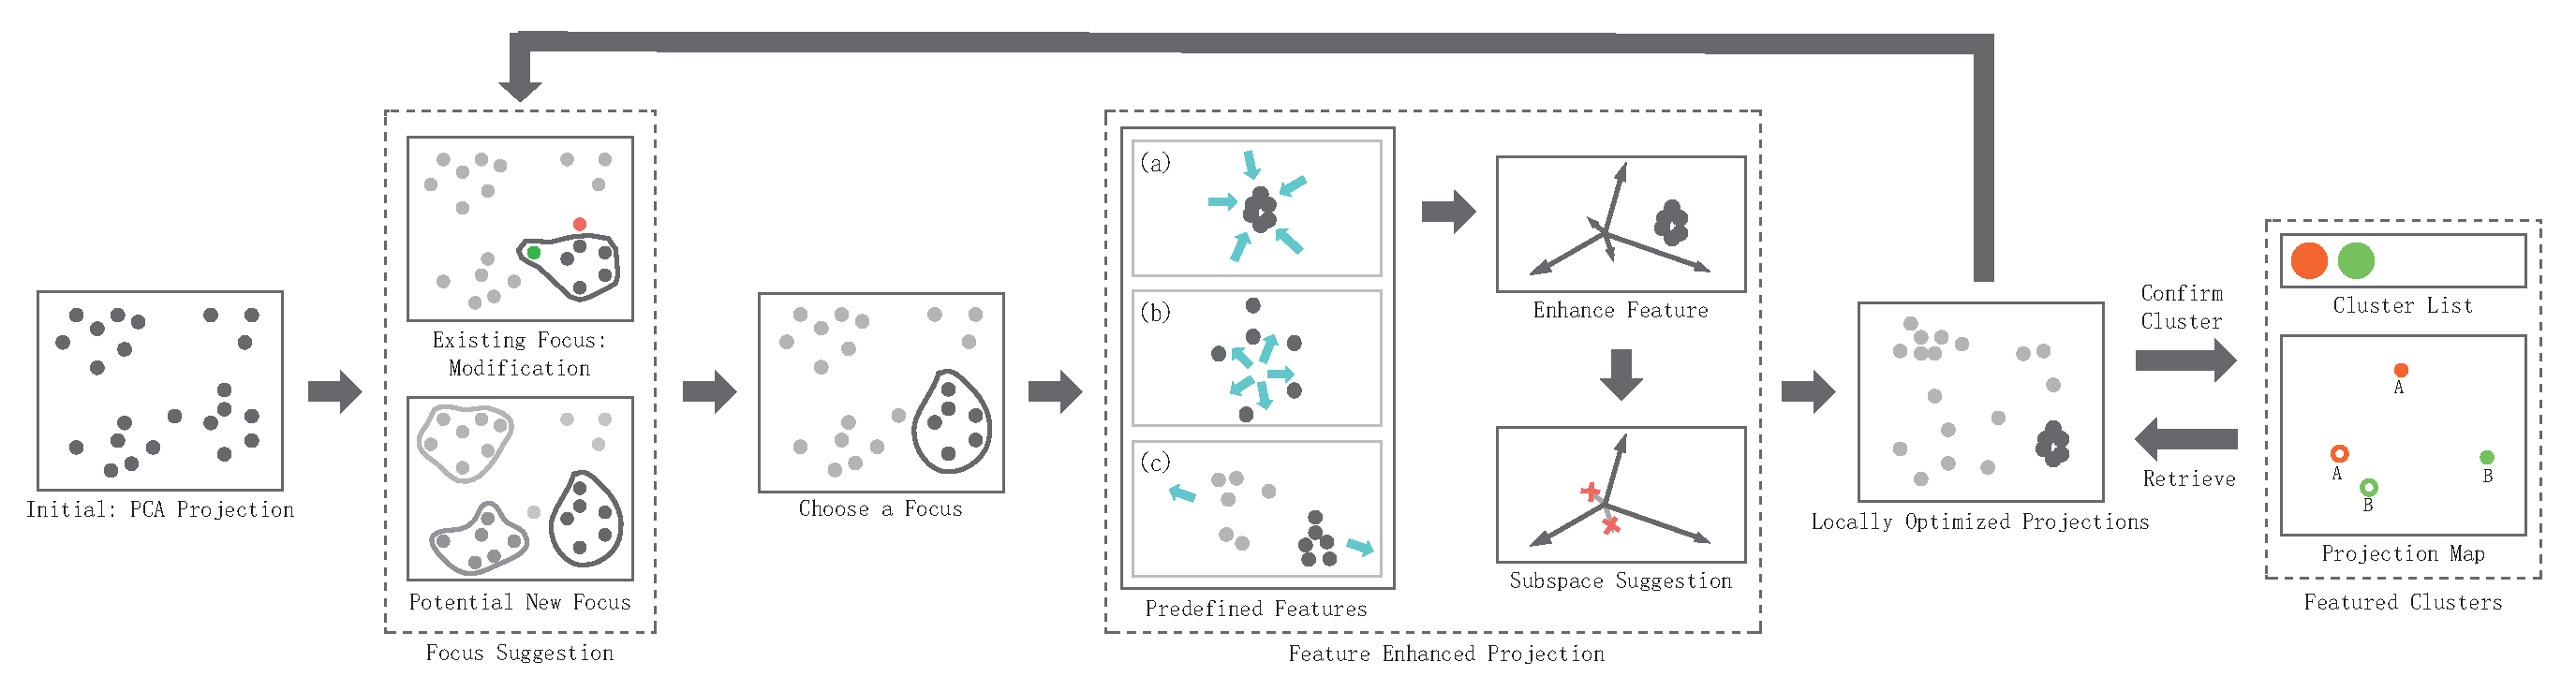
\includegraphics[width=1\linewidth]{images/Pipeline.eps}% 1\linewidth
  \caption{The overview of delivery system.}\label{fig.2}
  \end{figure*}
  \fi